\documentclass[]{article}
\usepackage{lmodern}
\usepackage{amssymb,amsmath}
\usepackage{ifxetex,ifluatex}
\usepackage{fixltx2e} % provides \textsubscript
\ifnum 0\ifxetex 1\fi\ifluatex 1\fi=0 % if pdftex
  \usepackage[T1]{fontenc}
  \usepackage[utf8]{inputenc}
\else % if luatex or xelatex
  \ifxetex
    \usepackage{mathspec}
  \else
    \usepackage{fontspec}
  \fi
  \defaultfontfeatures{Ligatures=TeX,Scale=MatchLowercase}
\fi
% use upquote if available, for straight quotes in verbatim environments
\IfFileExists{upquote.sty}{\usepackage{upquote}}{}
% use microtype if available
\IfFileExists{microtype.sty}{%
\usepackage{microtype}
\UseMicrotypeSet[protrusion]{basicmath} % disable protrusion for tt fonts
}{}
\usepackage[margin=1in]{geometry}
\usepackage{hyperref}
\hypersetup{unicode=true,
            pdftitle={统计的显著性水平},
            pdfauthor={侃侃迩行},
            pdfborder={0 0 0},
            breaklinks=true}
\urlstyle{same}  % don't use monospace font for urls
\usepackage{longtable,booktabs}
\usepackage{graphicx,grffile}
\makeatletter
\def\maxwidth{\ifdim\Gin@nat@width>\linewidth\linewidth\else\Gin@nat@width\fi}
\def\maxheight{\ifdim\Gin@nat@height>\textheight\textheight\else\Gin@nat@height\fi}
\makeatother
% Scale images if necessary, so that they will not overflow the page
% margins by default, and it is still possible to overwrite the defaults
% using explicit options in \includegraphics[width, height, ...]{}
\setkeys{Gin}{width=\maxwidth,height=\maxheight,keepaspectratio}
\IfFileExists{parskip.sty}{%
\usepackage{parskip}
}{% else
\setlength{\parindent}{0pt}
\setlength{\parskip}{6pt plus 2pt minus 1pt}
}
\setlength{\emergencystretch}{3em}  % prevent overfull lines
\providecommand{\tightlist}{%
  \setlength{\itemsep}{0pt}\setlength{\parskip}{0pt}}
\setcounter{secnumdepth}{0}
% Redefines (sub)paragraphs to behave more like sections
\ifx\paragraph\undefined\else
\let\oldparagraph\paragraph
\renewcommand{\paragraph}[1]{\oldparagraph{#1}\mbox{}}
\fi
\ifx\subparagraph\undefined\else
\let\oldsubparagraph\subparagraph
\renewcommand{\subparagraph}[1]{\oldsubparagraph{#1}\mbox{}}
\fi

%%% Use protect on footnotes to avoid problems with footnotes in titles
\let\rmarkdownfootnote\footnote%
\def\footnote{\protect\rmarkdownfootnote}

%%% Change title format to be more compact
\usepackage{titling}

% Create subtitle command for use in maketitle
\newcommand{\subtitle}[1]{
  \posttitle{
    \begin{center}\large#1\end{center}
    }
}

\setlength{\droptitle}{-2em}
  \title{统计的显著性水平}
  \pretitle{\vspace{\droptitle}\centering\huge}
  \posttitle{\par}
  \author{侃侃迩行}
  \preauthor{\centering\large\emph}
  \postauthor{\par}
  \predate{\centering\large\emph}
  \postdate{\par}
  \date{2017-08-11}

\usepackage{ctex}  
%\setCJKmainfont{文泉驿微米黑}  % 字体可以更换
\setCJKmainfont{Source Han Sans CN}  % Chinese font

\begin{document}
\maketitle

提高某些领域研究可重复性的一个直接和简单的方法是提高假设检验的统计显著性水平。

\hypertarget{hypothesis-testing}{%
\section{1. 统计检验和显著性水平}\label{hypothesis-testing}}

统计检验中,研究者最终希望确定零假设 (\(H_{i,i=0}\)) 和备择假设
(\(H_{i, i \neq 0}\))
中哪一个正确。由于这两种状态的不相容性,事实情况只有两种:要么是零假设正确;要么是其中一个备择假设如
\(H_1\)
正确。让事情变得更为复杂的是,研究者用于判断哪个假设正确的证据并不来自于数据整体,而来自于整体数据的一部分,即一个样本。样本统计量对于总体参数来说始终存在一定偏差,即抽样误差。

第一、零假设正确。假定零假设 (\(H_0\)) 整体服从平均值为 \(\mu_0 = 0\),
标准差为 \(\sigma = 1\)
的正态分布。即使在该零假设正确的前提下,由于抽样误差的原因,一个样本量为
\(n=1\) 的随机样本的样本平均值 (\(\overline{X}_i\)) 理论上来说可以是位于
\([-\infty, +\infty]\)
之间的任何一个数。但是从概率上来讲,样本平均值在总体平均值 0
的位置出现的概率最高;一个位置离总体平均值越远,样本平均值在该位置出现的概率就越低。例如,一个样本平均值出现在
\(\pm 3\) 位置上的概率就非常低了。
以样本平均值的大小为横坐标,该样本平均值出现的概率为纵坐标,可以画出如下样本平均值的概率密度分布图。

\begin{center}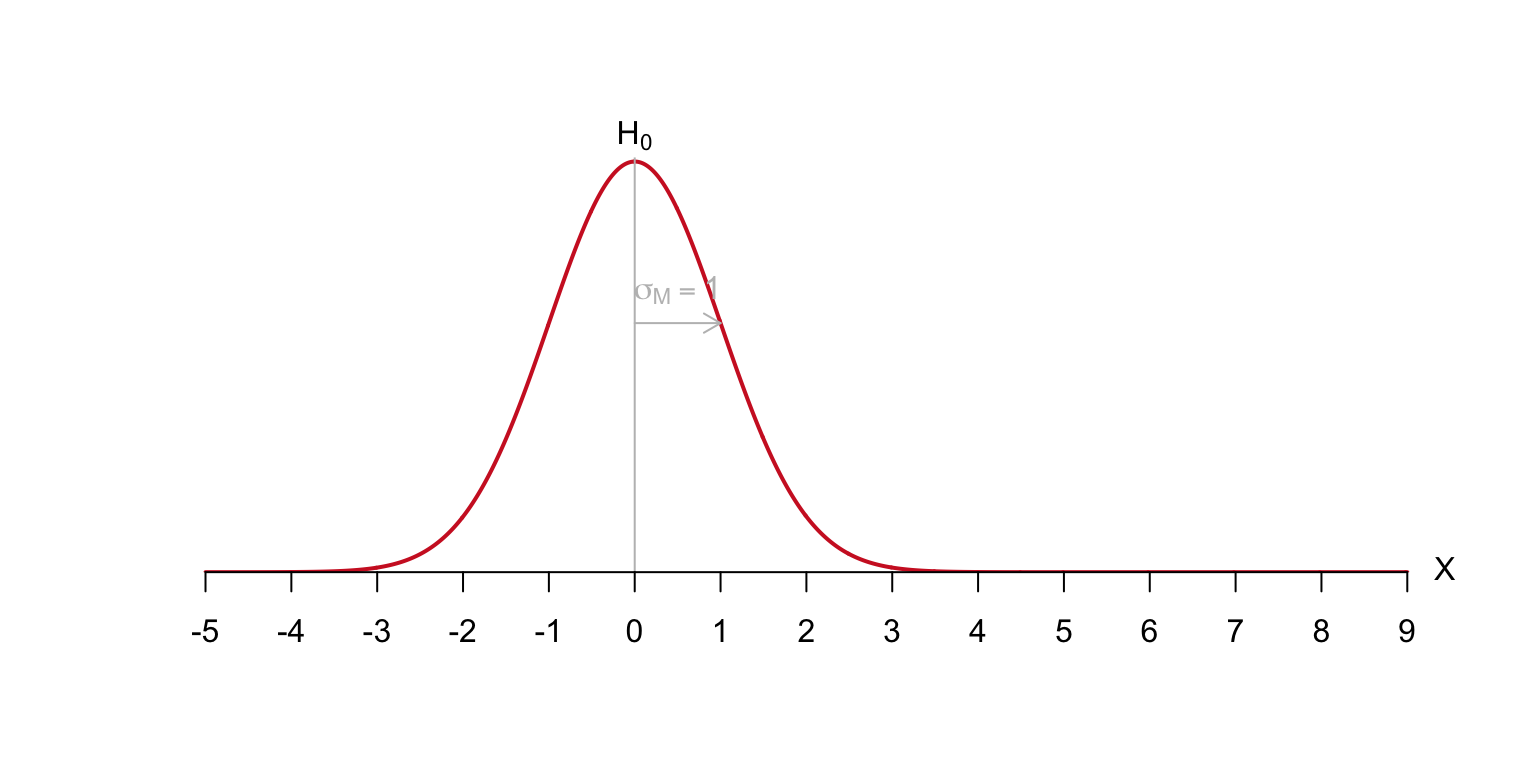
\includegraphics{2017-08-11-p-values-bayes-factor_files/figure-latex/Figure_1_01-1} \end{center}

\emph{P}-值指在零假设正确的前提下,样本平均值 (\(\overline{X}_i\))
与某个观测值 (\(\overline{X}_\text{obs}\))
一样极端或者比观测值更极端的概率。如观测值
(\(\overline{X}_\text{obs} = -1\)) 对应的 \emph{P} 值为 \(P=0.16\)。

\begin{center}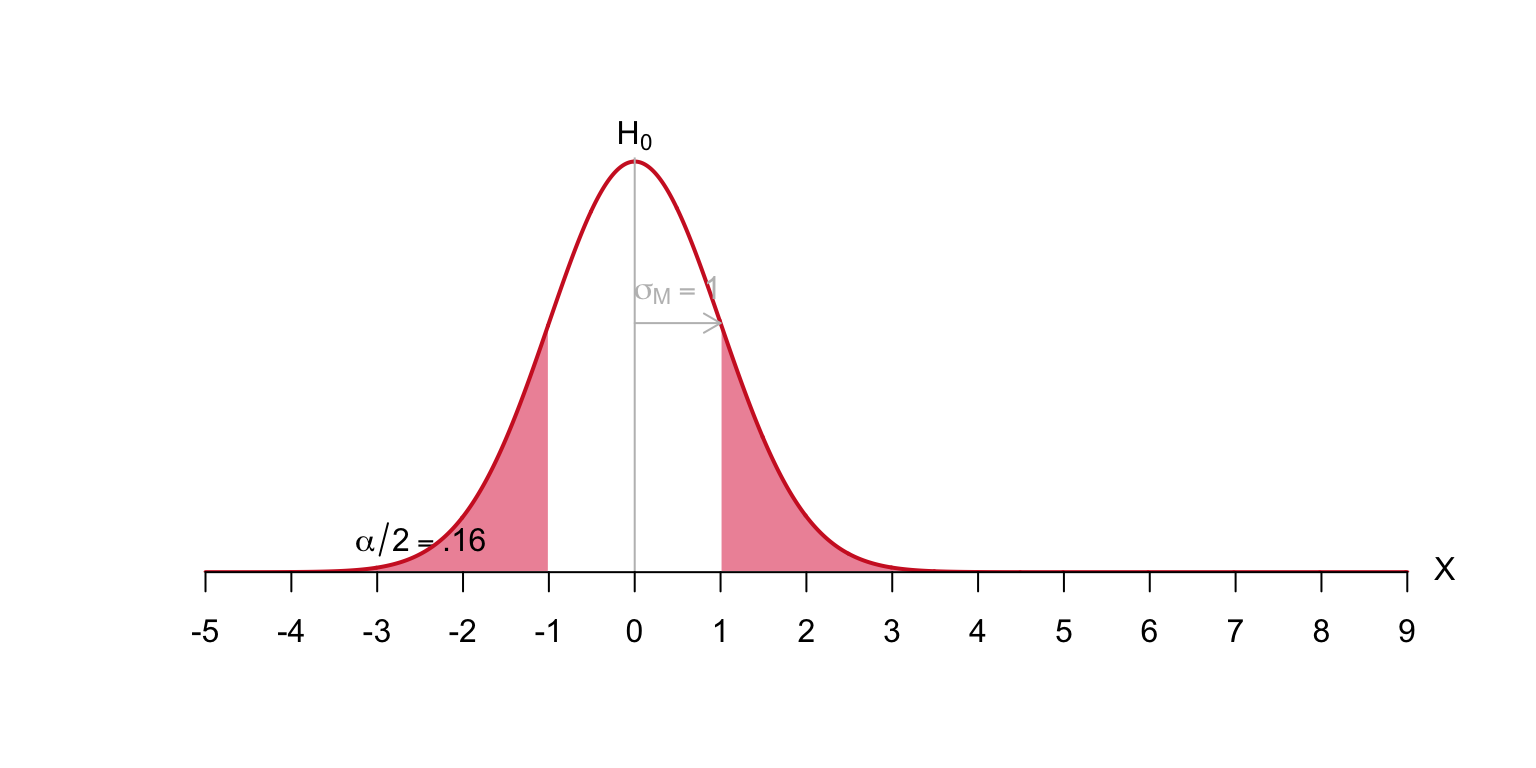
\includegraphics{2017-08-11-p-values-bayes-factor_files/figure-latex/Figure_1_02-1} \end{center}

如前所述,一个位置离总体平均值越远,样本平均值在该位置出现的概率就越低。当一个实际观测值
(\(\overline{X}_\text{obs}\))
离总体平均值足够远的时候,我们就有理由怀疑该样本不是来自零假设条件下的总体,而是来自于另外一个总体了。这个人为设定的\textbf{足够远},即为
\(\alpha\) 水平。心理学学家通常把该临界值定为 \(\alpha=0.05\)
(如下图)。如果观测值 (\(\overline{X}_\text{obs}\)) 大于等于 1.96, 即
\(|\overline{X}_\text{obs}|\geq 1.96\),或其在分布中出现的概率小于等于
0.05,
研究者则断定该样本并不来自于零假设整体,而是来自某个备择假设整体。如图所示,\(\alpha\)
水平又等价于当零假设实际上正确,但研究者拒绝零假设的概率,即 \textbf{I
类错误水平}。

\begin{center}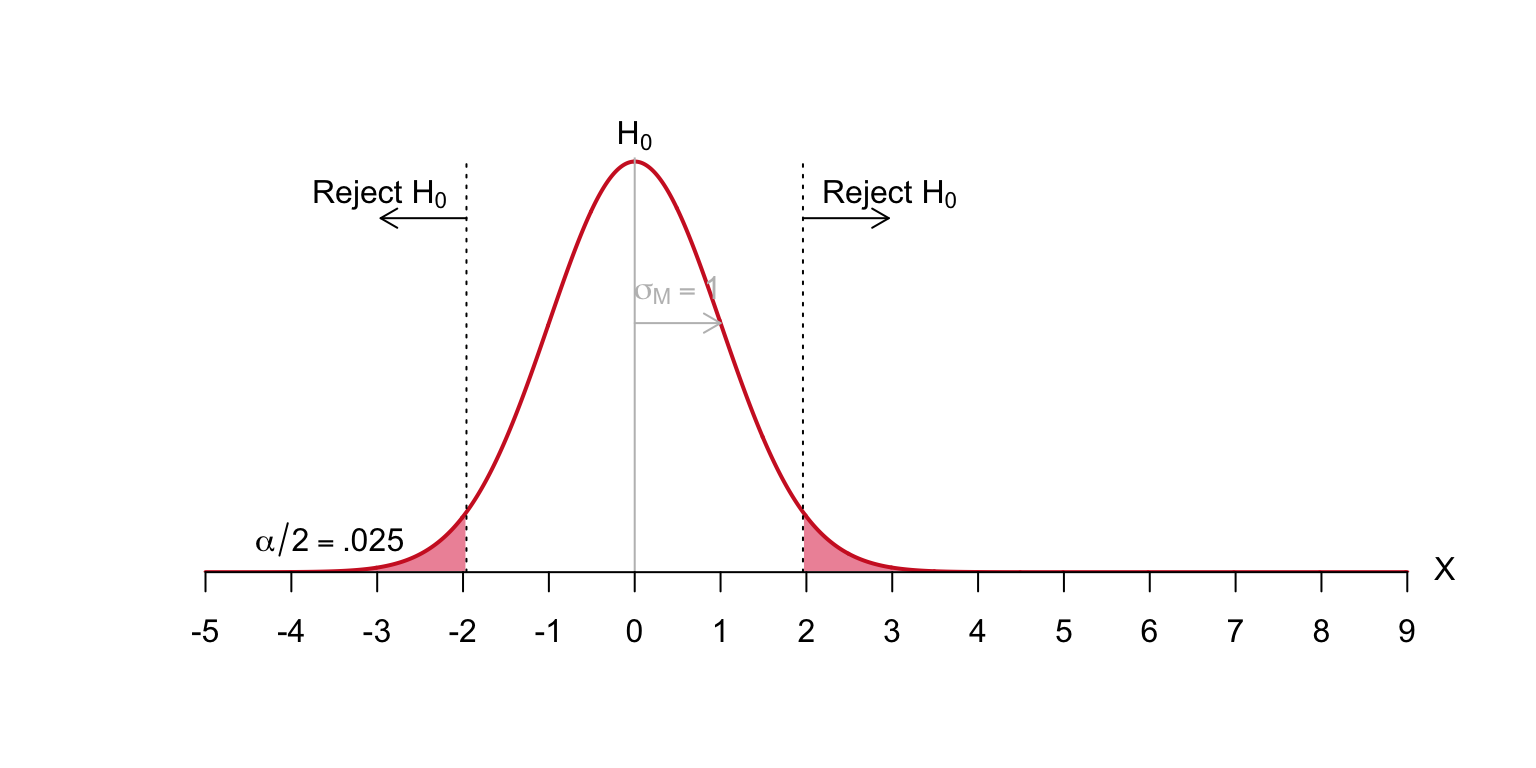
\includegraphics{2017-08-11-p-values-bayes-factor_files/figure-latex/Figure_1_03-1} \end{center}

第二、假设事实情况是零假设 (\(H_0\)) 错误,备择假设 (\(H_1\))
正确。同时假定零假设 (\(H_0\)) 和备择假设 (\(H_1\)) 间效应值大小为
\(\text{Cohen's D} = 4\),即备择假设 (\(H_1\)) 整体服从平均值为
\(\mu_0 = 4\), 标准差为 \(\sigma = 1\)
的正态分布。如果依然把显著性水平定为 \(\alpha=0.05\),即当
\(P \leq 0.05\) 或观测值 \(\overline{X}_{obs} \geq 1.96\)
时,拒绝零假设。 因为实际情况是备择假设 (\(H_1\)) 正确
(如下图),此时样本平均值 (\(\overline{X}_i\)) 有 \(1-\beta=0.98\)
的可能性位于临界值 1.96 的右侧,另有 \(\beta = 0.021\)
的可能性位于临界值的左侧。所以当 \(\overline{X}_{obs} \geq 1.96\)
时,如果我们拒绝零假设(\(H_0\)),接受备则假设
\(H_1\),那么我们的判断正确的概率是
\(1-\beta = 0.98\)。正确拒绝零假设的概率,\(1-\beta\) 又被称作统计效力
(statistical power)。因为在备择假设 (\(H_1\)) 正确的前提下,样本平均值
(\(\overline{X}_i\)) 仍有 \(\beta = 0.021\)
的可能性位于临界值的左侧。所以当观测值位于临界值左侧
\(\overline{X}_{obs} < 1.96\),我们的结论是无法拒绝零假设时,我们有
\(\beta = 0.021\) 的可能性是错的。此时研究者犯的是 \textbf{II
类错误},即实际上零假设 \(H_0\) 错误,备择假设 \(H_1\)
正确,但根据观测数据研究者无法拒绝零假设的情况。如图所示,II
类错误的概率是 \(\beta\)。

\begin{center}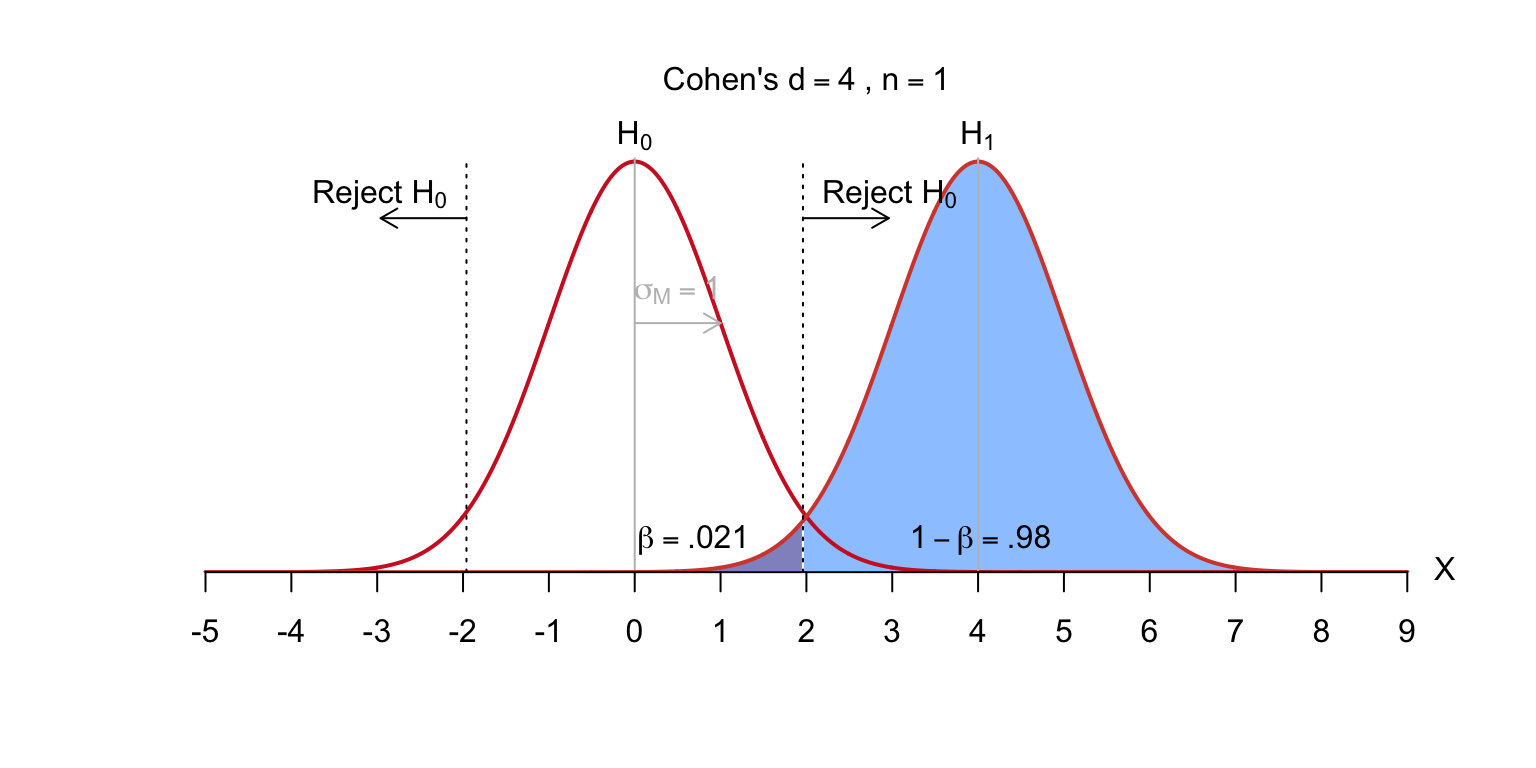
\includegraphics{2017-08-11-p-values-bayes-factor_files/figure-latex/Figure_1_04-1} \end{center}

上述四种情况可以总结为下面这个表格:

\begin{longtable}[]{@{}lcc@{}}
\toprule
& \(H_0\) & \(H_1\)\tabularnewline
\midrule
\endhead
没有拒绝零假设 & 正确拒斥(\(1-\alpha\)) &
漏报(II类错误,\(\beta\)值)\tabularnewline
拒绝零假设 & 虚报(I类错误,\(\alpha\)值) &
击中(统计效力,\(1-\beta\))\tabularnewline
\bottomrule
\end{longtable}

以及下面这个图:

\begin{center}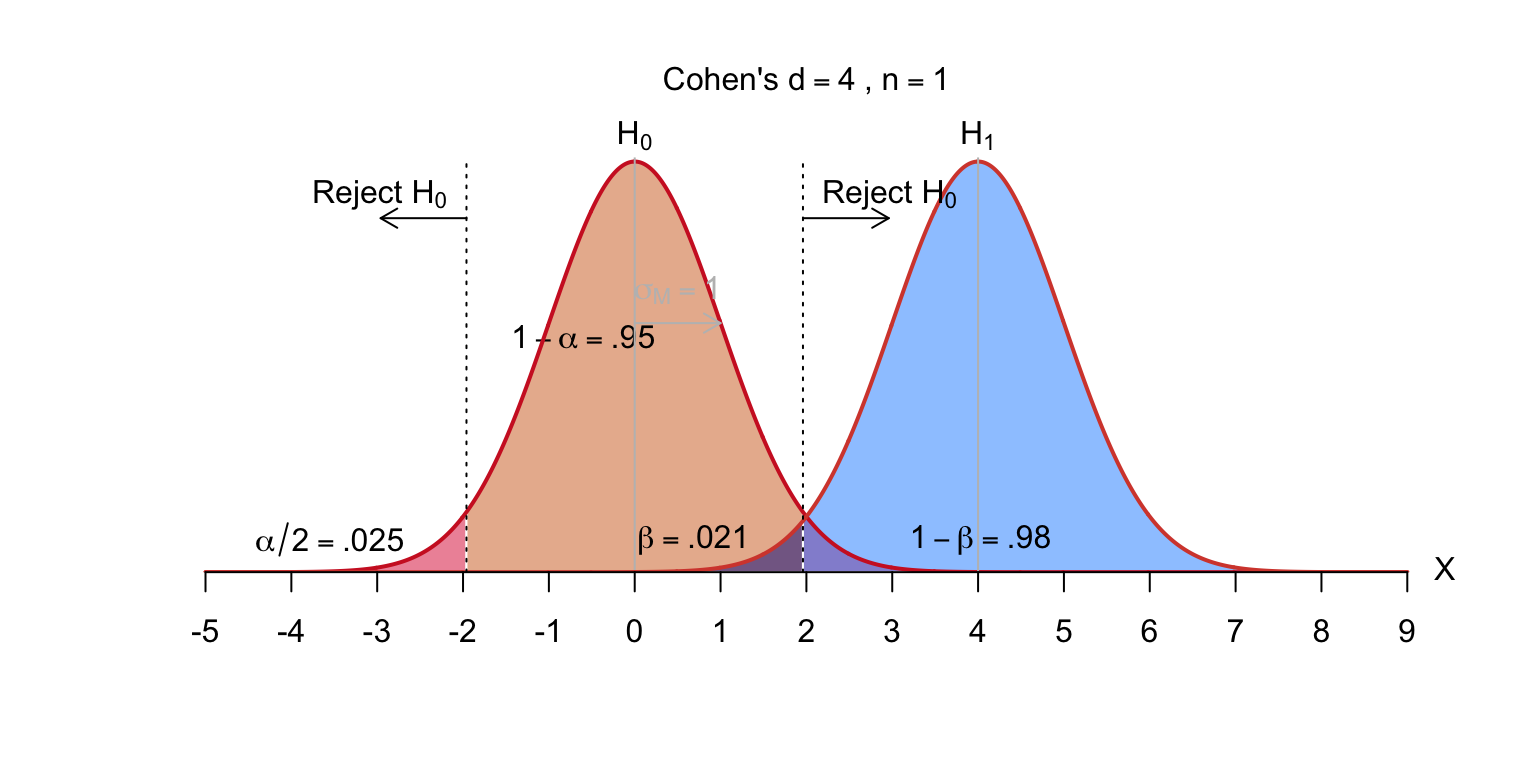
\includegraphics{2017-08-11-p-values-bayes-factor_files/figure-latex/Figure_1_05-1} \end{center}

\hypertarget{bf}{%
\section{2. 显著性水平和贝叶斯因子}\label{bf}}

如前所述,\emph{P} 值指在零假设 (\(H_0\))
正确的条件下,研究者记录到某个观测值 (\(\overline{X}_{obs}\)) 的概率,即
\(Pr(\overline{X}_{obs}|H_0)\)。而研究者关心的是记录到该观测值时零假设或备择假设正确与否的概率,即\(Pr(H_0|\overline{X}_{obs})\)
或 \(Pr(H_1|\overline{X}_{obs})\)
概率的大小。大多数情况下,研究者通常无法以一种二元论的方式去确定零假设还是备择假设正确,而只能从概率上哪讲哪个假设正确的可能性更大。判断哪个可能性更大的更直接证据来自于备择假设
\(H_1\) 和零假设 \(H_0\) 发生概率的比率
(Odds)。如下图所示,根据贝叶斯原则,在观测值 \(\overline{X}_{obs}\)
条件下,备择假设和零假设发生率之比受\textbf{贝叶斯因子} (Bayes factor,
\textbf{BF}) 和\textbf{先验概率} (prior odds) 两个因素的共同影响。

\[
\frac{\text{Pr }(H_1|\overline{X}_{obs})}{\text{Pr }(H_0|\overline{X}_{obs})}=
\frac{\text{Pr }(\overline{X}_{obs}|H_1)}{\text{Pr }(\overline{X}_{obs}|H_0)}\times
\frac{\text{Pr }(H_1)}{\text{Pr }(H_0)}=
BF \times (\text{prior odds})
\]

第一,关于备择假设和零假设发生概率之比的\textbf{先验知识} (prior odds)
通常来源于研究者的前期假设、相关领域科学研究的共识、或同领域相似研究问题的其他研究。通常认为,心理学研究和癌症临床研究中,备择假设和零假设的先验比率约为
\textbf{1:10}。而在前临床的生物医学研究 (preclinical biomedical
reaearch) 领域,该先验比率会更低。

第二、
\textbf{贝叶斯因子}来源于观测数据,贝叶斯因子的大小表明了证据的强度。贝叶斯因子越大,观测数据越有能力支持备择假设假设。按照
Kass 和 Raftery (1995) 的观点,贝叶斯因子的大小和证据强度 (strength of
evidence) 存在以下关系:

\begin{longtable}[]{@{}cc@{}}
\toprule
贝叶斯因子大小 & 否定零假设的证据强度\tabularnewline
\midrule
\endhead
1-3.2 & 不值一提\tabularnewline
3.2-10 & 显著的 (Substantial)\tabularnewline
10-100 & 强 (Strong)\tabularnewline
\textgreater{}100 & 确定的 (Decisive)\tabularnewline
\bottomrule
\end{longtable}

贝叶斯因子和 \emph{P}-值之间的关系受备择假设的影响。要确定贝叶斯因子和
\emph{P}-值之间的关系,首先要确定备择假设 \(\overline{H}_{i,i\neq0}\)
的分布特征。确定备择假设的方法不同,计算出的贝叶斯因子和
\emph{P}-值的关系也不同。如果我们假定备择假设和零假设条件下整体分布的形状一致,那么确定备择假设的分布特征就是确定其整体平均值
\(\mu_1\)。

\begin{itemize}
\tightlist
\item
  第一种方法利用显著性检验中的\textbf{统计效力}大小确定备择假设的整体平均值。例如,备择假设整体平均值
  \(\mu_1\) 的大小必须让被则假设满足其统计效力为
  75\%。根据统计效力大小确定备择假设后,观察到的
  \emph{P}-值大小和贝叶斯因子大小之间的关系叫做 \textbf{效力曲线}
  (power)。
\end{itemize}

\begin{center}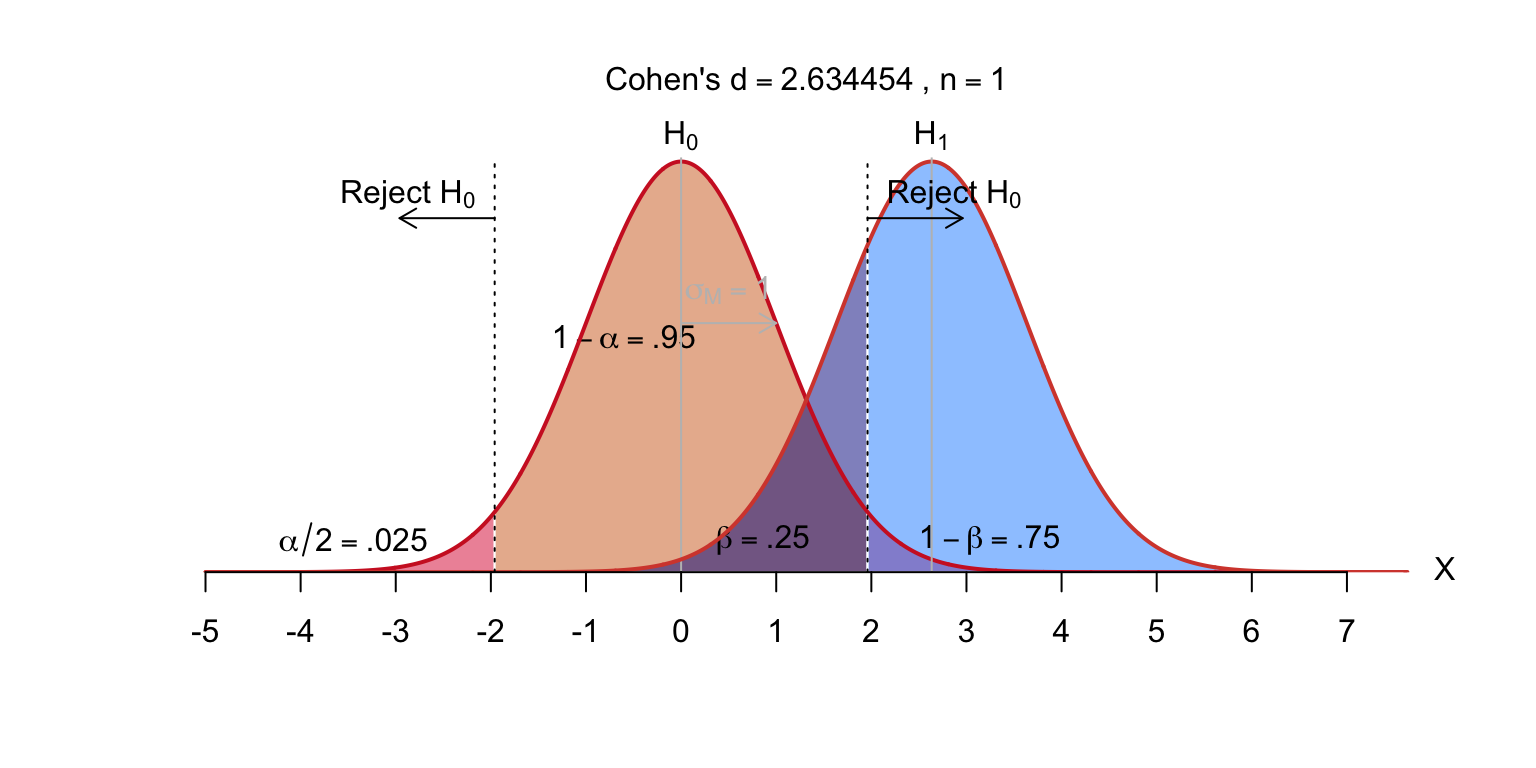
\includegraphics{2017-08-11-p-values-bayes-factor_files/figure-latex/Figure_1_06-1} \end{center}

\begin{itemize}
\tightlist
\item
  第二种方法是通过显著性水平来确定备择假设的整体平均值的。Johnson (2013)
  认为备择假设的整体平均值应该设定在 \(\alpha/2 = 0.0025\)
  处。这种方法叫做\textbf{均匀最大功效贝叶斯检验} (Uniformly Most
  Powerful Bayesian Test, UMPBT)。在我们的例子中,零假设为真时
  \(\alpha/2 = 0.0025\) 对应的 \(\overline{X}_{obs}=\)
  2.81,所以备择假设的整体平均值为 \(\mu_1=\)
  2.81。因为当备择假设的整体平均值为 \(\mu_1=\) 2.81
  时,显著性检验的统计效力为
  \(1-\beta=0.80\),所以该方法确定的备择假设与第一种方法中把统计效力设定为
  \(80\%\) 时的出来的 \(P\)-值和贝叶斯因子之间的关系是一样的。
\end{itemize}

\begin{center}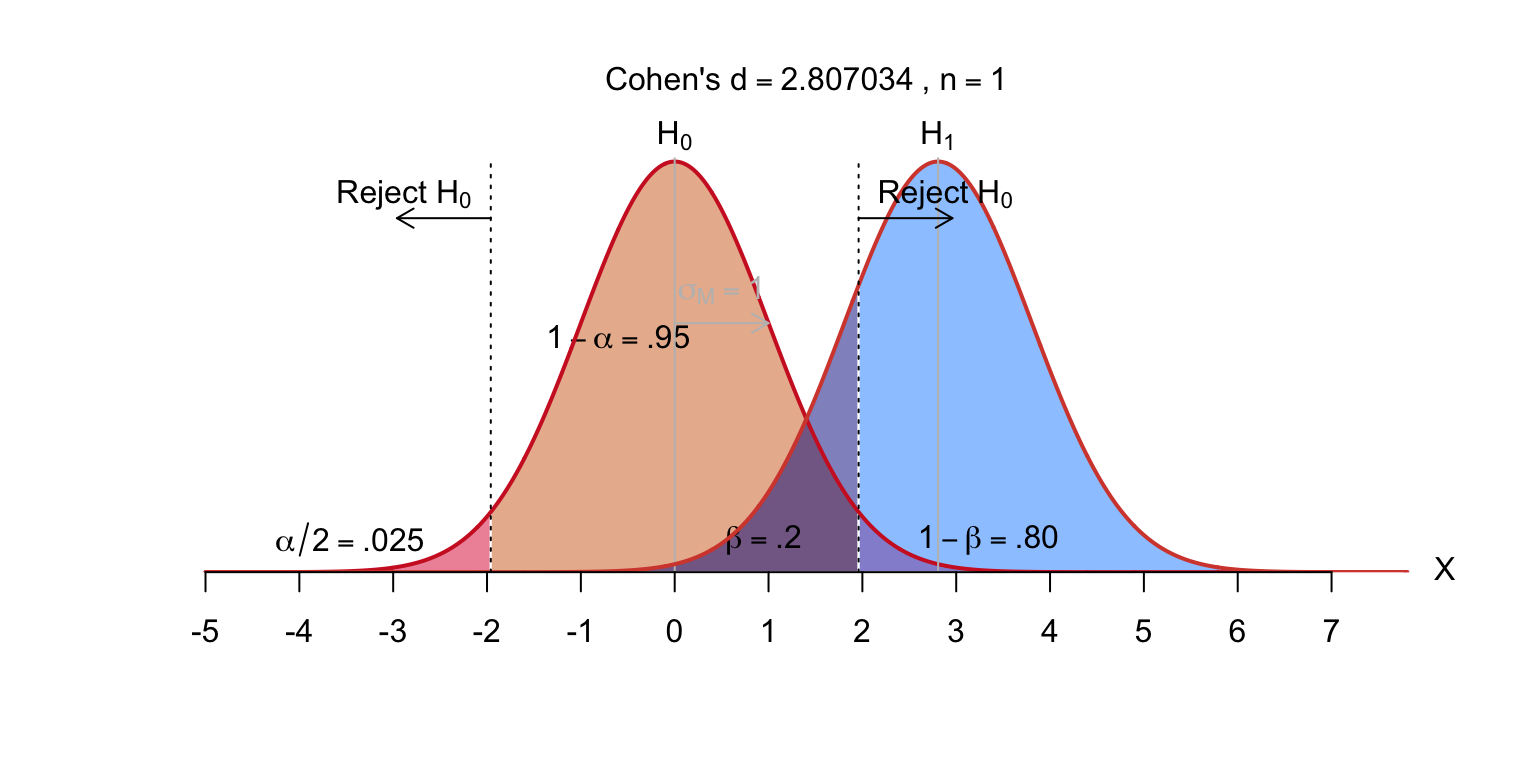
\includegraphics{2017-08-11-p-values-bayes-factor_files/figure-latex/Figure_1_07-1} \end{center}

后两种方法没有试图找到一个特定备择假设,而是在假定备择假设具有某种特点时,去描述
\emph{P}-值和贝叶斯因子的关系。

\begin{itemize}
\tightlist
\item
  第三种方法认为如果备择假设 \(H_{i}\) 的整体平均值 \(\mu_i\) 以零假设
  \(H_{i, i=0}\) 的整体平均值 \(\mu_0\)
  为中心的对称分布时,那么贝叶斯因子的上限将不超过
  \(BF = 1/(2\times \exp(\frac{1}{2}t^2))\),此处 \(t\) 指 I
  类错误的大小。此种方法被称作 \textbf{似然值比率范围} (likelihood ratio
  bound) (Berger, \& Sellke, 1987)
\item
  第四种方法认为当备择假设 \(H_{i}\) 的整体平均值 \(\mu_i\)
  是一个以零假设 \(H_{i, i=0}\) 的整体平均值 \(\mu_0\) 为众数的单峰分布
  (unimodal),并满足某些限制条件时,贝叶斯因子的上限将不超过
  \(BF=1/(-\exp(1) \cdot p \ \cdot \ln(p))\),\(p\) 即为
  \(p\)-值的大小。此方法被称作\textbf{局部 \(H_1\) 范围} (Local-\(H_1\)
  Bound) (Sellke, Bayarri, \& Berger, 2001)
\end{itemize}

用上述四种方法确定备择假设或者假定备择假设具有某种特征后,\emph{P}-值和贝叶斯因子的关系可以用下图表示(Benjamin
et al., 2017):

\begin{center}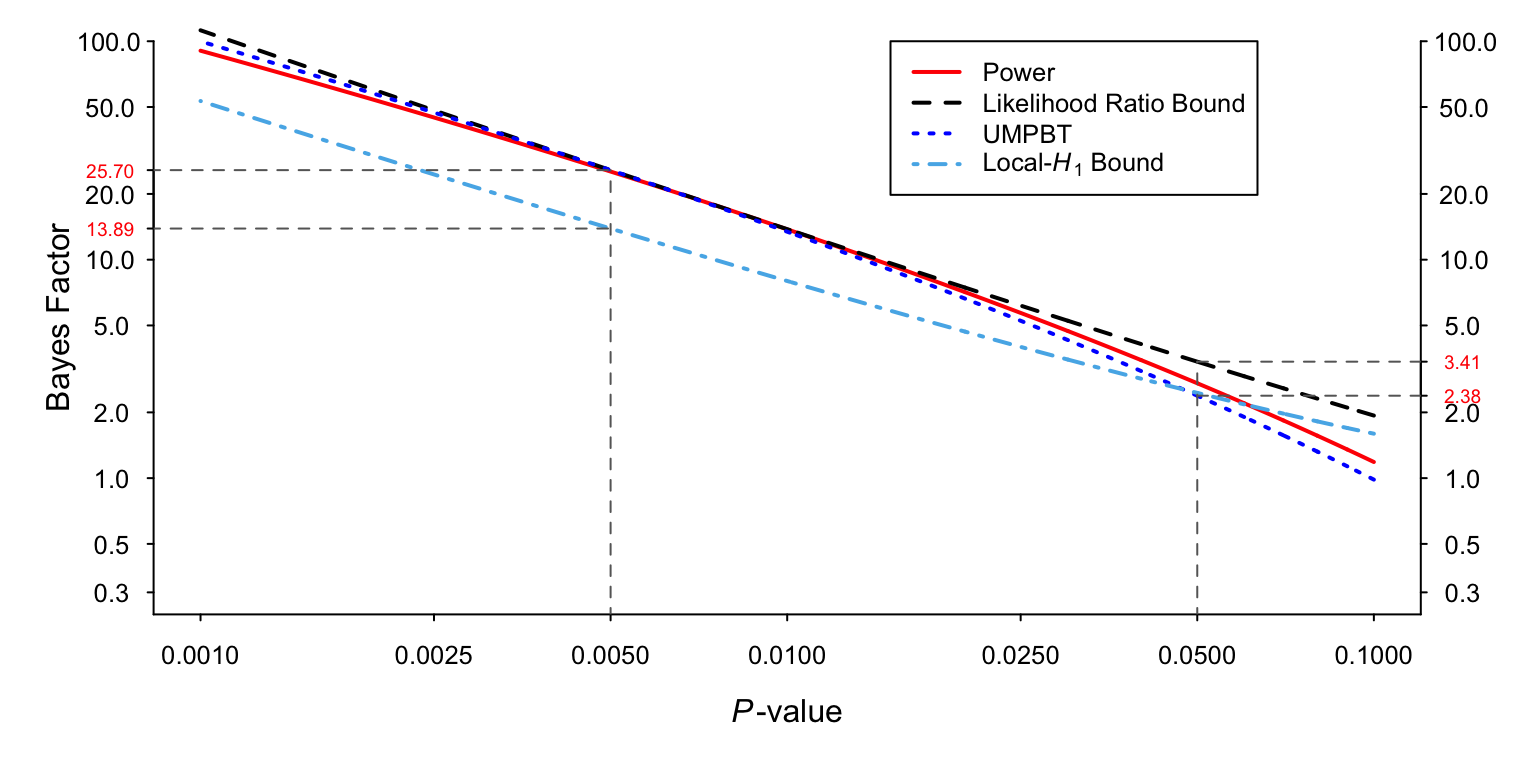
\includegraphics{2017-08-11-p-values-bayes-factor_files/figure-latex/Figure_2_01-1} \end{center}

如上图所示,显著性水平为 \(P < .05\) 的双尾检验所对应的贝叶斯因子仅为
\(2.5 - 3.4\)。根据前面的描述,此时否定零假设的证据是非常弱的。如果我们把研究的先验概率设定为
\(1:10\),此时备择假设发生的可能性仅为零假设发生可能性的三分之一,即
\(\frac{1}{3} = 3.4 \times \frac{1}{10}\)。而当我们把显著性水平设定为
\(p < .005\) 的水平上时,贝叶斯因子就增加到了
\(13.80-25.70\)。根据前述标准,此时证据力度是很强的。在同样的先验概率下,备择假设和零假设的比率增加到了
\(2.57\)。

\hypertarget{fpr}{%
\section{3. 显著性水平和假阳性率}\label{fpr}}

在贝叶斯框架下,\emph{P}-值的一个对应替代方案是\textbf{假阳性率}(false
positive
rate,FPR)。错误发现率指在所有零假设被拒绝的情景中,零假设实际上为真的概率。假设一项研究中,零假设
(\(H_0\)) 为真的概率为 \(\phi\),备择假设 (\(H_i\)) 为真概率则为
\(1-\phi\)。如果把假设检验的临界值设定为 \(\alpha\), 即当
\(P < \alpha\) 时拒绝零假设 (\(H_0\))。因为零假设发生的概率是
\(\phi\),那么研究者错误拒绝零假设的概率为
\(\alpha\phi\)。另外如果该假设检验的统计效力为
\(1-\beta\),那么研究者正确拒绝零假设的概率为 \((1-\beta)(1-\phi)\)。
此时错误发现率可以表示为错误决绝零假设的概率与所有拒绝零假设的概率的比率,如下图:

\[
\text{false positive rate} \approx
\frac
{\alpha\phi}
{\alpha\phi + (1-\beta)(1-\alpha)}
\]

如上面的公式所示,假阳性率同时受显著性水平、先验概率和统计效力的共同影响。在选取了三个先验概率水平
\(1:40\)、\(1:10\) 和 \(1:5\),两个显著性水平 \(P <.05\) 和 \(p <.005\)
后,我们可以看到假阳性率和统计效力存在下图所示的关系:

\begin{center}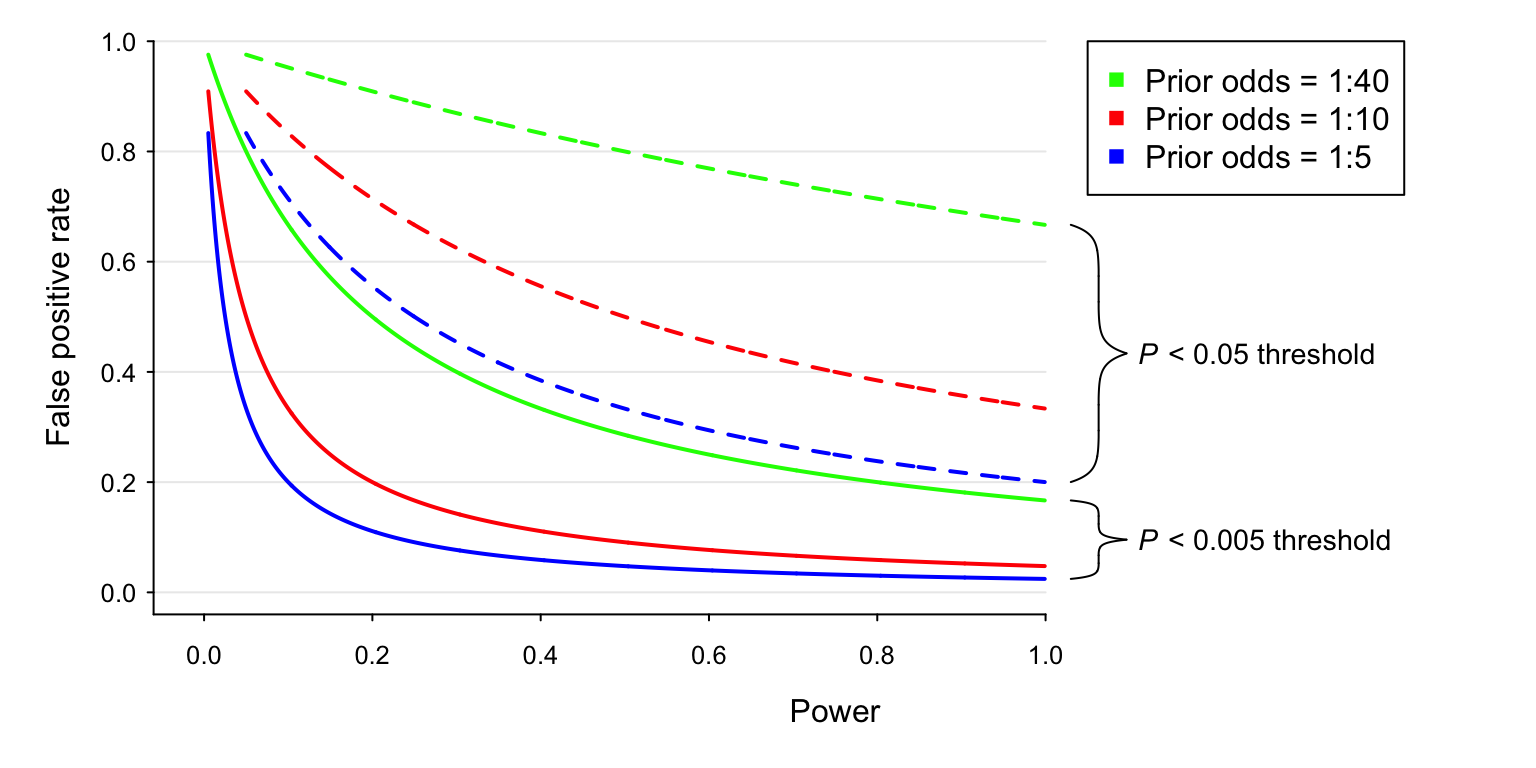
\includegraphics{2017-08-11-p-values-bayes-factor_files/figure-latex/Figure_3_01-1} \end{center}

如上图所示,低统计效力加上低显著性水平 \(\alpha = 0.05\)
将产生高比率的假阳性率。如果显著性水平设置为
\(P < 0.05\),先验概率设定为
\emph{1:10},那么无论统计效力处于什么水平,该分析的假阳性率将\textbf{不低于
33\%}。心理学及许多科学研究的一个事实是统计效力都比较低。而如果把显著性水提高到
\emph{0.005},则在绝大部分统计效力范围内,假阳性率可降到 \(5\%\) 之下。

\hypertarget{power}{%
\section{4. 显著性水平和统计效力}\label{power}}

提高统计显著性水平的缺点也是显而易见的,即提高统计的显著性水平将显著降低假设检验的统计效力、提高
II 类错误的概率。如下图所示,在 \(\alpha=0.05\)
的显著性水平下,该显著性检验的统计效力为 \(1-\beta=0.80\) 。

\begin{center}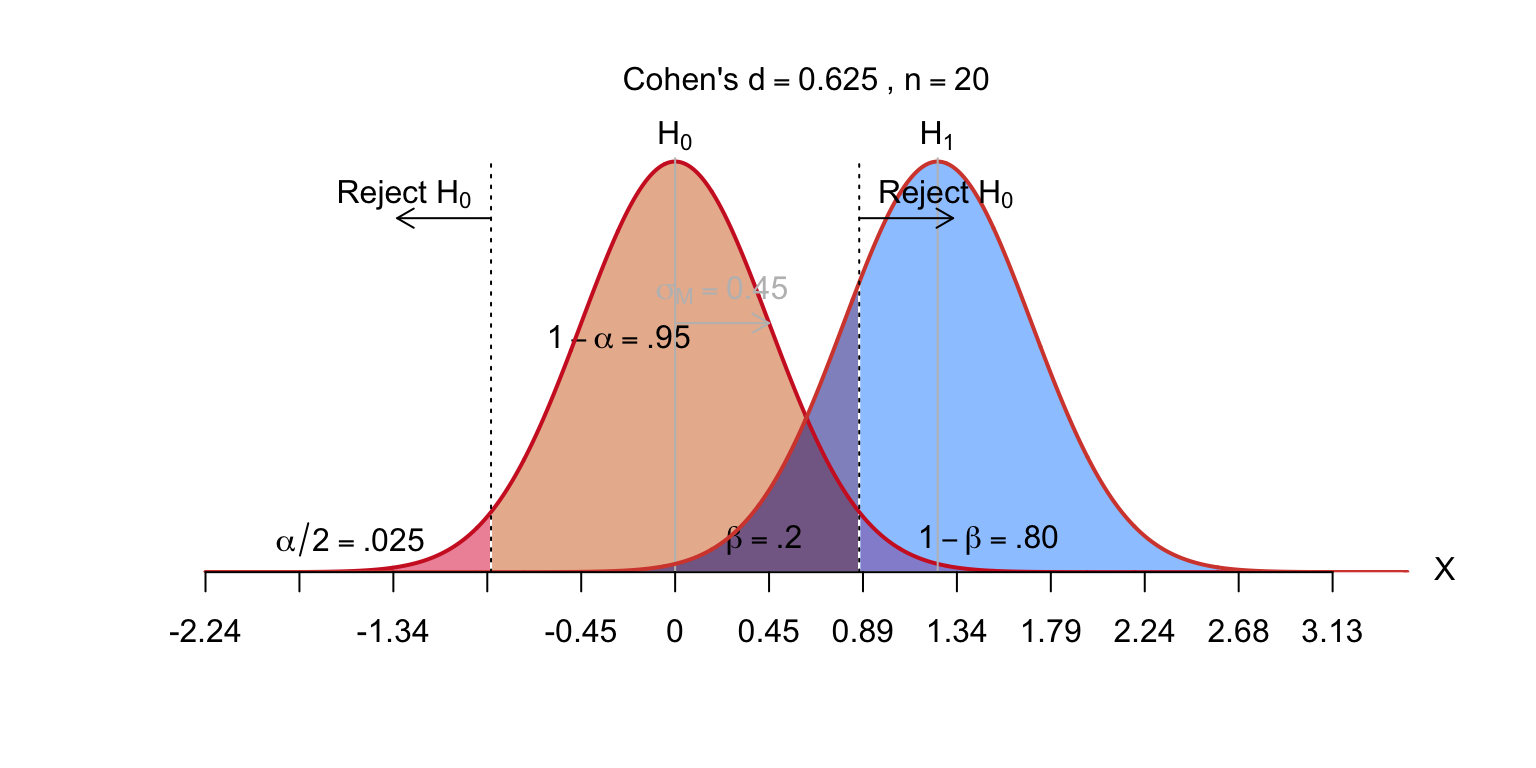
\includegraphics{2017-08-11-p-values-bayes-factor_files/figure-latex/Figure_1_08-1} \end{center}

但当我们把统计显著性提高到 \(\alpha=0.005\)
时,该检验的统计效力就降低到了 \(1-\beta=0.50\)。

\begin{center}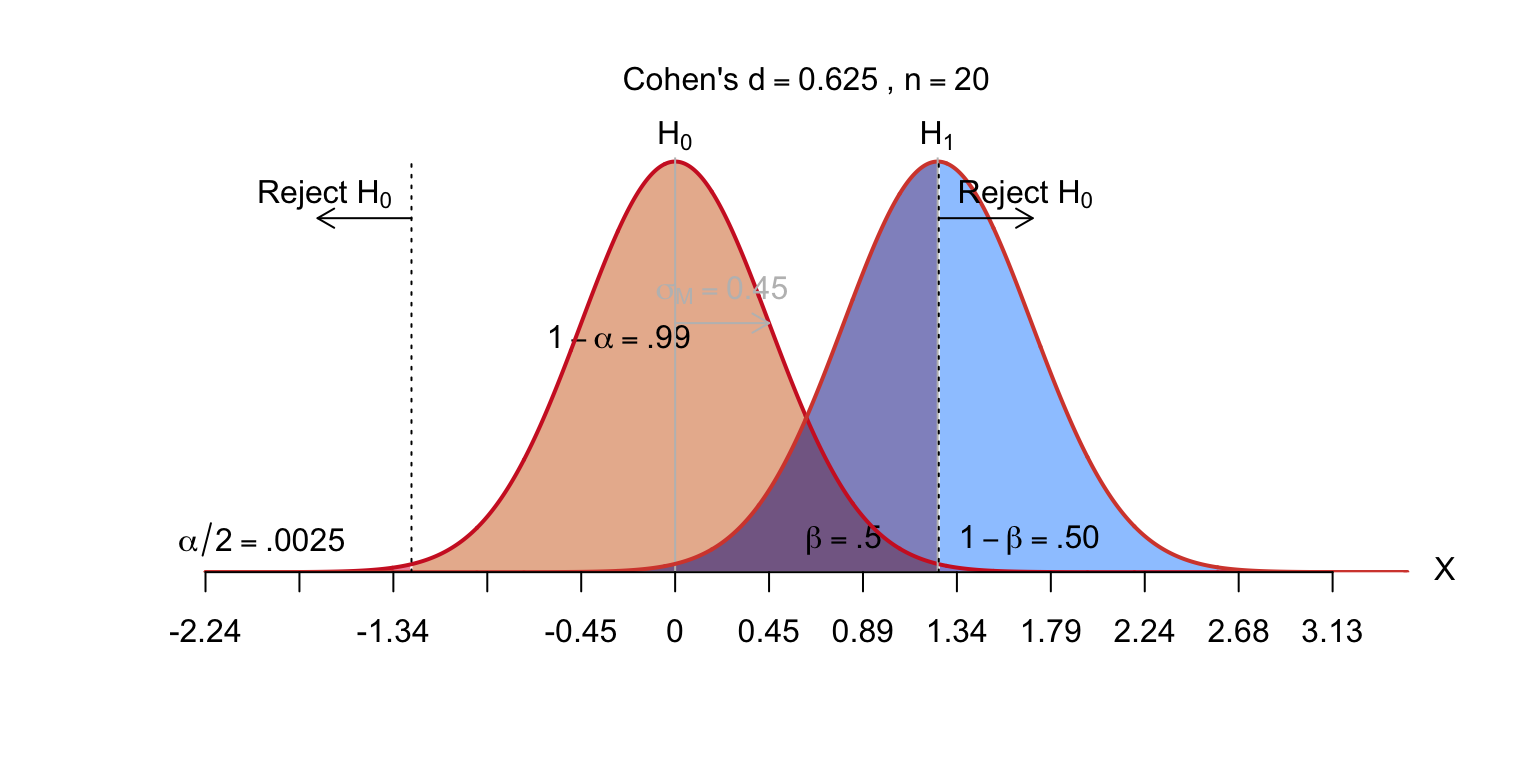
\includegraphics{2017-08-11-p-values-bayes-factor_files/figure-latex/Figure_1_09-1} \end{center}

此时,如果想保持原来的统计效力水平,研究者就需要提高研究的样本量(实际应用中,这将增加项目的研究成本)。如下图所示,如果我们把样本量增加
70\%,检验的统计效力将恢复到 \(1-\beta=0.80\) 的水平。

\begin{center}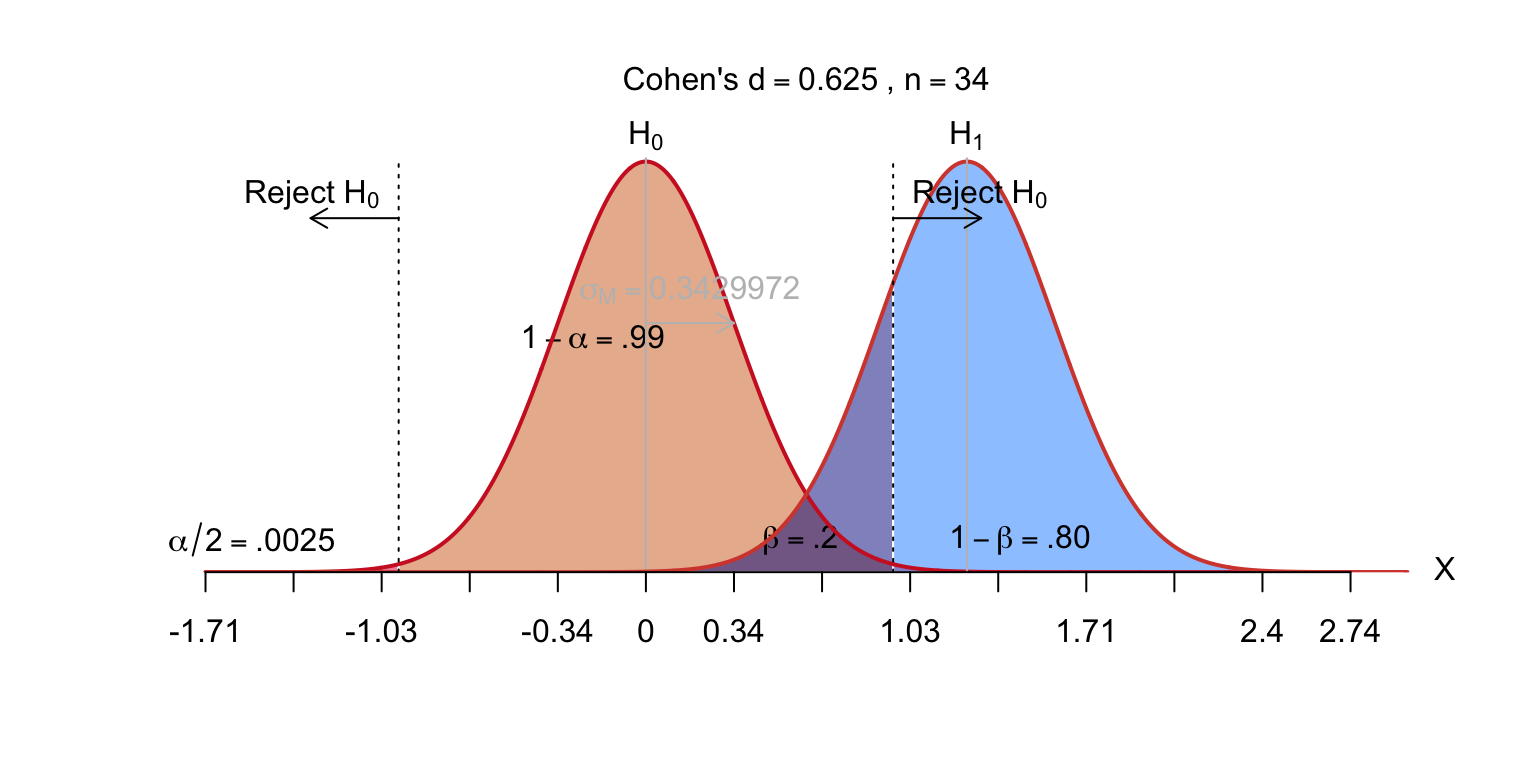
\includegraphics{2017-08-11-p-values-bayes-factor_files/figure-latex/Figure_1_10-1} \end{center}

\hypertarget{summary}{%
\section{5. 总结}\label{summary}}

如前所述,提高假设检验中的统计显著性水平能显著提高统计检验的贝叶斯因子水平、显著降低统计检验的假阳性率。在实践中,提高统计显著性水平也能显著提高科学研究的可重复性
(Benjamin et al., 2017)。正是基于上述原因,目前有 72
为统计学家联名发文希望在传统上使用两个标准差 (\(\alpha = .05\))
作为显著性水平的研究领域应该把显著性水平提高到三个标准差
(\(\alpha = .005\)) (Benjamin et al., 2017)。

在某些先验概率非常低的探索性研究领域,研究者需要远比 0.005
更为严苛的显著性水平。如通常认为基因和高能物理研究领域的显著性水平应该符合五个标准差原则
(5-sigma),即显著性水平大约为 \(P < 3\times 10^{-7}\)。

提高统计的显著性水平并不是解决研究可重复性问题的唯一方法。其他可能的解决方案包括选择更为合适的统计方法,如模型比较和贝叶斯学习等、更周到的实验设计、预实验等等。当然,改变
\emph{P}-值的显著性水平最为直接和最为简单的方法。

\hypertarget{references}{%
\section{6. 参考文献}\label{references}}

Altman, N., \& Krzywinski, M. (2017). Points of Significance:
Interpreting P values. \emph{Nature Methods, 14}(3), 213-214.
\url{doi:10.1038/nmeth.4210}

Benjamin, D. J., et al.,. (2017). Redefine Statistical Significance.
\emph{Nature Human Behavior}. \url{doi:10.1038/s41562-017-0189-z}

Berger, J. O., \& Sellke, T. (1987). Testing a Point Null Hypothesis:
The Irreconcilability of P Values and Evidence. \emph{Journal of the
American Statistical Association, 82}(397), 112-122.

Chawla, D. S. (2017). P-value shake-up proposed. \emph{Nature, 548},
16-17. \url{doi:10.1038/nature.2017.22375}

Johnson, V. E. (2013). Revised standards for statistical evidence.
\emph{Proceedings of the National Academy of Sciences of the United
States of America, 110}(48), 19313-19317.
\url{doi:10.1073/pnas.1313476110}

Kass, R. E., \& Raftery, A. E. (1995). Bayes Factors. \emph{Journal of
the American Statistical Association, 90}(430), 773-795.
\url{doi:10.1080/01621459.1995.10476572}

Nuzzo, B. (2014). Statistical errors. \emph{Nature, 506}, 150-152.
\url{doi:http://doi.org/10.1038/506150a}

Sellke, T., Bayarri, M. J., \& Berger, J. O. (2001). Calibration of p
Values for Testing Precise Null Hypotheses. \emph{The American
Statistician, 55}(1), 62-71. \url{doi:10.1198/000313001300339950}

Wasserstein, R. L., \& Lazar, N. A. (2016). The ASA`s Statement on
p-Values: Context, Process, and Purpose. \emph{The American
Statistician, 70}(2), 129-133. \url{doi:10.1080/00031305.2016.1154108}


\end{document}
